% This file was created by matplotlib2tikz v0.6.18.
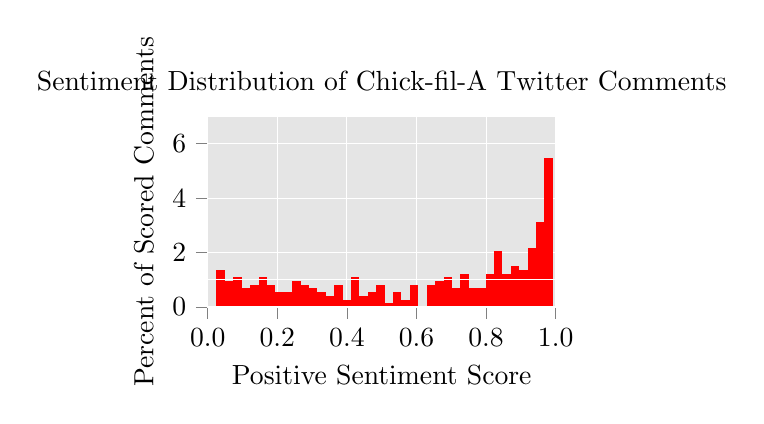
\begin{tikzpicture}

\begin{axis}[
axis background/.style={fill=white!89.80392156862746!black},
axis line style={white},
height=4cm,
tick align=outside,
tick pos=left,
title={Sentiment Distribution of Chick-fil-A Twitter Comments},
width=6cm,
x grid style={white},
xlabel={Positive Sentiment Score},
xmajorgrids,
xmin=0, xmax=1,
xtick={0,0.2,0.4,0.6,0.8,1},
xticklabels={0.0,0.2,0.4,0.6,0.8,1.0},
y grid style={white},
ylabel={Percent of Scored Comments},
ymajorgrids,
ymin=0, ymax=7
]
\draw[fill=red,draw opacity=0] (axis cs:0.0251235365867615,0) rectangle (axis cs:0.0492905825376511,1.36563226856155);
\draw[fill=red,draw opacity=0] (axis cs:0.0492905825376511,0) rectangle (axis cs:0.0734576284885406,0.95594266167118);
\draw[fill=red,draw opacity=0] (axis cs:0.0734576284885406,0) rectangle (axis cs:0.0976246744394302,1.09250589905278);
\draw[fill=red,draw opacity=0] (axis cs:0.0976246744394302,0) rectangle (axis cs:0.1217917278409,0.682815976399201);
\draw[fill=red,draw opacity=0] (axis cs:0.121791735291481,0) rectangle (axis cs:0.145958781242371,0.81937967690028);
\draw[fill=red,draw opacity=0] (axis cs:0.145958751440048,0) rectangle (axis cs:0.170125797390938,1.09250589905278);
\draw[fill=red,draw opacity=0] (axis cs:0.170125812292099,0) rectangle (axis cs:0.19429287314415,0.819378919068656);
\draw[fill=red,draw opacity=0] (axis cs:0.19429287314415,0) rectangle (axis cs:0.218459919095039,0.546252949526388);
\draw[fill=red,draw opacity=0] (axis cs:0.218459904193878,0) rectangle (axis cs:0.242626950144768,0.546252949526388);
\draw[fill=red,draw opacity=0] (axis cs:0.24262697994709,0) rectangle (axis cs:0.26679402589798,0.955943251096321);
\draw[fill=red,draw opacity=0] (axis cs:0.266793996095657,0) rectangle (axis cs:0.290961056947708,0.819378919068656);
\draw[fill=red,draw opacity=0] (axis cs:0.290961056947708,0) rectangle (axis cs:0.315128117799759,0.682815765890547);
\draw[fill=red,draw opacity=0] (axis cs:0.315128087997437,0) rectangle (axis cs:0.339295119047165,0.546253286340755);
\draw[fill=red,draw opacity=0] (axis cs:0.339295148849487,0) rectangle (axis cs:0.363462209701538,0.409689459534328);
\draw[fill=red,draw opacity=0] (axis cs:0.363462209701538,0) rectangle (axis cs:0.387629240751266,0.819379929511133);
\draw[fill=red,draw opacity=0] (axis cs:0.387629240751266,0) rectangle (axis cs:0.411796301603317,0.273126306356219);
\draw[fill=red,draw opacity=0] (axis cs:0.411796271800995,0) rectangle (axis cs:0.435963302850723,1.09250657268151);
\draw[fill=red,draw opacity=0] (axis cs:0.435963332653046,0) rectangle (axis cs:0.460130393505096,0.409689459534328);
\draw[fill=red,draw opacity=0] (axis cs:0.460130393505096,0) rectangle (axis cs:0.484297424554825,0.546253286340755);
\draw[fill=red,draw opacity=0] (axis cs:0.484297394752502,0) rectangle (axis cs:0.508464455604553,0.819379929511133);
\draw[fill=red,draw opacity=0] (axis cs:0.508464455604553,0) rectangle (axis cs:0.532631516456604,0.136563153178109);
\draw[fill=red,draw opacity=0] (axis cs:0.532631516456604,0) rectangle (axis cs:0.556798577308655,0.546252612712437);
\draw[fill=red,draw opacity=0] (axis cs:0.556798577308655,0) rectangle (axis cs:0.580965638160706,0.273126306356219);
\draw[fill=red,draw opacity=0] (axis cs:0.580965638160706,0) rectangle (axis cs:0.605132699012756,0.819378919068656);
\draw[fill=red,draw opacity=0] (axis cs:0.605132699012756,0) rectangle (axis cs:0.629299700260162,0);
\draw[fill=red,draw opacity=0] (axis cs:0.629299700260162,0) rectangle (axis cs:0.653466761112213,0.819378919068656);
\draw[fill=red,draw opacity=0] (axis cs:0.653466761112213,0) rectangle (axis cs:0.677633821964264,0.955942072246765);
\draw[fill=red,draw opacity=0] (axis cs:0.677633821964264,0) rectangle (axis cs:0.701800882816315,1.09250522542487);
\draw[fill=red,draw opacity=0] (axis cs:0.70180082321167,0) rectangle (axis cs:0.725967824459076,0.682817449963418);
\draw[fill=red,draw opacity=0] (axis cs:0.725967884063721,0) rectangle (axis cs:0.750134944915771,1.22906837860298);
\draw[fill=red,draw opacity=0] (axis cs:0.750134944915771,0) rectangle (axis cs:0.774302005767822,0.682815765890547);
\draw[fill=red,draw opacity=0] (axis cs:0.774302005767822,0) rectangle (axis cs:0.798469066619873,0.682815765890547);
\draw[fill=red,draw opacity=0] (axis cs:0.798469066619873,0) rectangle (axis cs:0.822636127471924,1.22906837860298);
\draw[fill=red,draw opacity=0] (axis cs:0.822636127471924,0) rectangle (axis cs:0.84680312871933,2.04845234989025);
\draw[fill=red,draw opacity=0] (axis cs:0.84680312871933,0) rectangle (axis cs:0.870970189571381,1.22906837860298);
\draw[fill=red,draw opacity=0] (axis cs:0.870970189571381,0) rectangle (axis cs:0.895137250423431,1.5021946849592);
\draw[fill=red,draw opacity=0] (axis cs:0.895137250423431,0) rectangle (axis cs:0.919304311275482,1.36563153178109);
\draw[fill=red,draw opacity=0] (axis cs:0.919304251670837,0) rectangle (axis cs:0.943471252918243,2.18501583988294);
\draw[fill=red,draw opacity=0] (axis cs:0.943471312522888,0) rectangle (axis cs:0.967638373374939,3.14095252309651);
\draw[fill=red,draw opacity=0] (axis cs:0.967638373374939,0) rectangle (axis cs:0.99180543422699,5.46252612712437);
\path [draw=white, fill opacity=0] (axis cs:0,0)
--(axis cs:0,7);

\path [draw=white, fill opacity=0] (axis cs:1,0)
--(axis cs:1,7);

\path [draw=white, fill opacity=0] (axis cs:0,0)
--(axis cs:1,0);

\path [draw=white, fill opacity=0] (axis cs:0,1)
--(axis cs:1,1);

\end{axis}

\end{tikzpicture}